\chapter{Numerical Results}

In this section, we will show our pricing results for square root mean-reverting model and one heston one CEV model. We use Monte Carlo simulations as our benchmark as there's no existing pricing formulas for these models.

\section{Volatility option prices under mean-reverting CEV model}

For options under mean-reverting CEV model, generally we use the same mean-reverting parameters as \cite{grunbichler_valuing_1996} used in his model, the parameters are $\kappa=4$, $\theta=2$, $K=0.15$. Besides, we set the nuisance parameter $\sigma_0 = \sigma_{\text{CEV}} v_0^{\gamma-\frac{1}{2}}$, where $v_0$ is the initial value of volatility. We test our approximation method with different constant elasticity parameters. To evaluate the accuracy of our method, we use Monte Carlo simulation's result with $200$ steps and $100000$ paths, and plot it versus results calculated by our approximation method with four corrective terms; We also follow \cite{kristensen_adding_2011} to plot percentage error to the corrective terms. Results of our method are shown to be very accurate. \footnote{Results can be found in Appendix \ref{mrcev}}{Figures are as following}:

\begin{figure}[!tbp]
    \centering
    \subfloat[delta comparison]{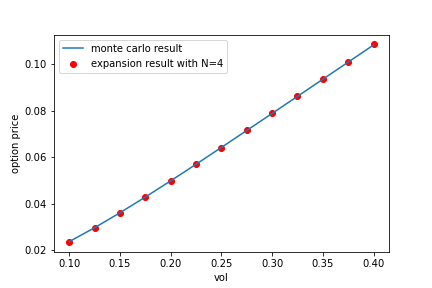
\includegraphics[width=0.5\textwidth]{./figures/T=0.3,K=0.15, kappa=4,m=0.2, sigma=0.15, gamma=0.3.csv price.png}\label{price comparison1}}
    \hfill
    \subfloat[delta differences between two methods]{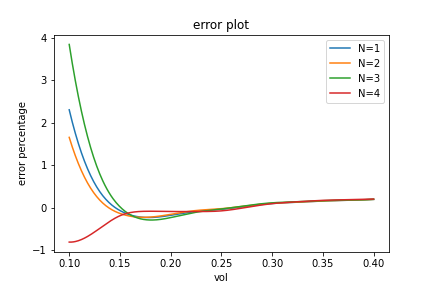
\includegraphics[width=0.5\textwidth]{./figures/T=0.3,K=0.15, kappa=4,m=0.2, sigma=0.15, gamma=0.3.csv error.png}\label{price diff1}}
    \caption{Parameters are $T=0.3,K=0.15, \kappa=4,\theta=0.2, \sigma=0.15, \gamma=0.3$}
  \end{figure}

\begin{figure}[!tbp]
\centering
\subfloat[Price comparison]{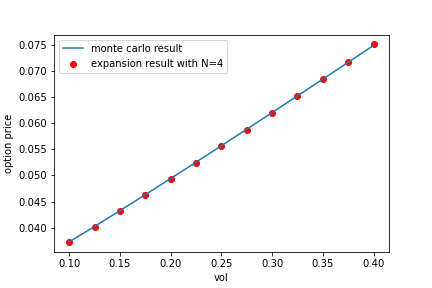
\includegraphics[width=0.5\textwidth]{./figures/T=0.5,K=0.15, kappa=4,m=0.2, sigma=0.15, gamma=0.3.csv price.png}\label{price comparison2}}
\hfill
\subfloat[Price percentage difference]{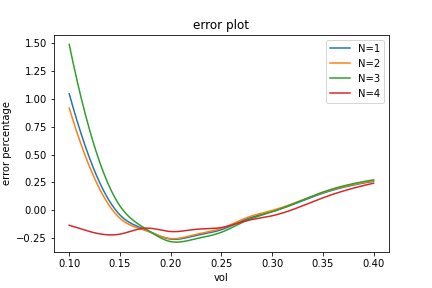
\includegraphics[width=0.5\textwidth]{./figures/T=0.5,K=0.15, kappa=4,m=0.2, sigma=0.15, gamma=0.3.csv error.png}\label{price diff2}}
\caption{Parameters are $T=0.5,K=0.15, \kappa=4,\theta=0.2, \sigma=0.15, \gamma=0.3$}
\end{figure}

\begin{figure}[!tbp]
\centering
\subfloat[Price comparison]{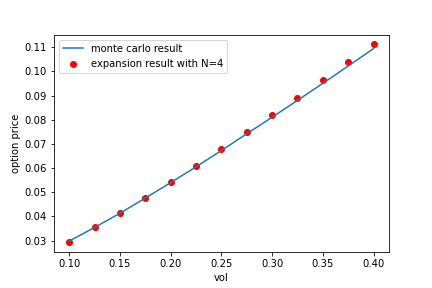
\includegraphics[width=0.5\textwidth]{./figures/T=0.3,K=0.15, kappa=4,m=0.2, sigma=0.6, gamma=0.75.csv price.png}\label{price comparison3}}
\hfill
\subfloat[Price percentage difference]{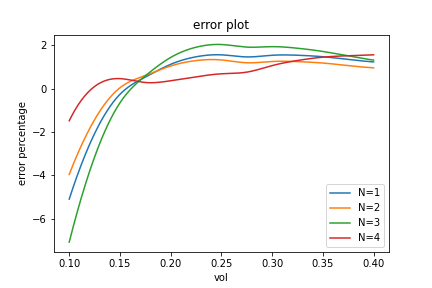
\includegraphics[width=0.5\textwidth]{./figures/T=0.3,K=0.15, kappa=4,m=0.2, sigma=0.6, gamma=0.75.csv error.png}\label{price diff3}}
\caption{Parameters are $T=0.3,K=0.15, \kappa=4,\theta=0.2, \sigma=0.6, \gamma=0.75$}
\end{figure}

\begin{figure}[!tbp]
    \centering
    \subfloat[Price comparison]{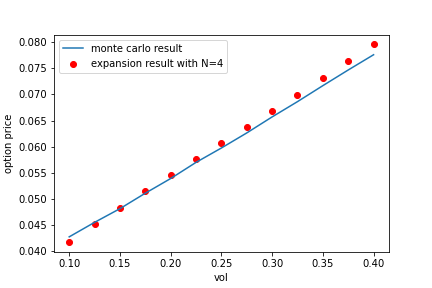
\includegraphics[width=0.5\textwidth]{./figures/T=0.5,K=0.15, kappa=4,m=0.2, sigma=0.6, gamma=0.75.csv price.png}\label{price comparison4}}
    \hfill
    \subfloat[Price percentage difference]{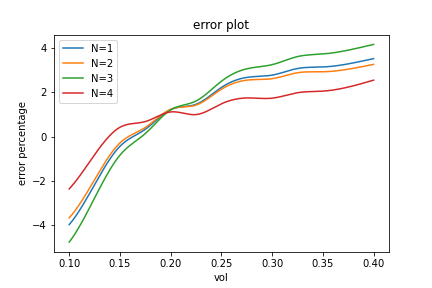
\includegraphics[width=0.5\textwidth]{./figures/T=0.5,K=0.15, kappa=4,m=0.2, sigma=0.6, gamma=0.75.csv error.png}\label{price diff4}}
    \caption{Parameters are $T=0.5,K=0.15, \kappa=4,\theta=0.2, \sigma=0.6, \gamma=0.75$}
\end{figure}